\documentclass[a4paper,11pt]{article}
\input{/home/tof/Documents/Cozy/latex-include/preambule_lua.tex}
\newcommand{\showprof}{show them}  % comment this line if you don't want to see todo environment
\fancyhead[L]{Requêtes avancées}
\newdate{madate}{10}{09}{2020}
%\fancyhead[R]{\displaydate{madate}} %\today
%\fancyhead[R]{Seconde - SNT}
%\fancyhead[R]{Première - NSI}
\fancyhead[R]{Terminale - NSI}
\fancyfoot[L]{~\\Christophe Viroulaud}
\AtEndDocument{\label{lastpage}}
\fancyfoot[C]{\textbf{Page \thepage/\pageref{lastpage}}}
\fancyfoot[R]{\includegraphics[width=2cm,align=t]{/home/tof/Documents/Cozy/latex-include/cc.png}}
\usepackage{tikz}

\begin{document}
\begin{Form}
\begin{commentprof}
toujours sur bd-avec-emprunts.db (version initiale: il y a eu des modifications dans le cours précédent)
\end{commentprof}
\section{Problématique}
Nous n'avons, pour l'instant, effectué que des requêtes simples et sur une seule table. Mais la puissance d'une base de données est de pouvoir mettre en relation de manière efficiente, des informations multiples. 
\begin{commentprof}
En gardant l'exemple de la base des bandes dessinées, il va être intéressant de pouvoir remplir la table des emprunts à partir des tables des emprunteurs et des bandes dessinées.
\end{commentprof}
\begin{center}
\shadowbox{\parbox{15cm}{\centering Comment effectuer des requêtes plus complexes pour mettre en relation plusieurs tables?}}
\end{center}
\section{Fonctions d'agrégation}
Ce sont des fonctions qui vont regrouper les lignes. La plupart des fonctions d'agrégation vont permettre de faire des statistiques sur les données. Le code \ref{count} compte le nombre de lignes (donc d'albums) de la série \emph{Aya de Yopougon}.
\begin{center}
\begin{lstlisting}[language=SQL]
SELECT COUNT(*) FROM Bandes_dessinees WHERE serie = "Aya de Yopougon";
\end{lstlisting}
\captionof{code}{Compter des lignes}
\label{count}
\end{center}

\begin{aretenir}[]
Le code suivant donnerait le même résultat que le code \ref{count}.
\begin{lstlisting}[language=SQL]
SELECT COUNT(titre) FROM Bandes_dessinees WHERE serie = "Aya de Yopougon";
\end{lstlisting}
Cependant si certaines lignes avaient un titre \emph{NULL} elles ne seraient ici pas comptées.
\end{aretenir}
Il existe de nombreuses fonctions d'agrégation. Citons la moyenne (\emph{AVG}), la somme (\emph{SUM}), le maximum (\emph{MAX}). La documentation en ligne détaillera de manière exhaustive ces fonctions.
\begin{activite}
\begin{enumerate}
\item Tester la requête \ref{count}.
\item Compter le nombre total de bandes dessinées.
\item Tester la requête \ref{distinct}. Que renvoie-t-elle?
\begin{center}
\begin{lstlisting}[language=SQL]
SELECT COUNT(DISTINCT id_dessinateur) FROM Bandes_dessinees;
\end{lstlisting}
\captionof{code}{Mot clé \emph{DISTINCT}}
\label{distinct}
\end{center}
\end{enumerate}
\end{activite}
\section{Mettre des tables en relation}
\subsection{Sous-requêtes}
La requête \ref{jeunesse} sélectionne toutes les bandes dessinées du genre \emph{Jeunesse}.
\begin{center}
\begin{lstlisting}[language=SQL]
SELECT titre FROM Bandes_dessinees WHERE id_genre = 13;
\end{lstlisting}
\captionof{code}{Bandes dessinées jeunesse}
\label{jeunesse}
\end{center}
Cependant il est nécessaire de connaître l'\emph{id} du genre \emph{Jeunesse} dans la table \emph{Genres}. La requête \ref{genre} récupère cet id.
\begin{center}
\begin{lstlisting}[language=SQL]
SELECT id FROM Genres WHERE genre = "Jeunesse";
\end{lstlisting}
\captionof{code}{id du genre Jeunesse}
\label{genre}
\end{center}
Il est possible de combiner ces deux requêtes.
\begin{center}
\begin{lstlisting}[language=SQL]
SELECT titre FROM Bandes_dessinees 
       WHERE id_genre = (SELECT id FROM Genres WHERE genre = "Jeunesse");
\end{lstlisting}
\captionof{code}{Sous-requête}
\label{sous}
\end{center}
\begin{activite}
\begin{enumerate}
\item Tester la requête \ref{sous}.
\item Sélectionner les titres de livres dessinés par Joann Sfar.
\item Compter les titres publiés par l'éditeur Delcourt.
\item Que renvoie la requête \ref{isbn}?
\begin{center}
\begin{lstlisting}[language=SQL]
SELECT titre FROM Bandes_dessinees WHERE isbn IN (SELECT isbn FROM Emprunts WHERE id_emprunteurs = 1);
\end{lstlisting}
\captionof{code}{Sous requête}
\label{isbn}
\end{center}
\end{enumerate}
\end{activite}
\subsection{Jointures}
Il existe des informations communes entre certaines tables. Une jointure permet de mettre en relation ces données (figure \ref{jointure}).
\begin{center}
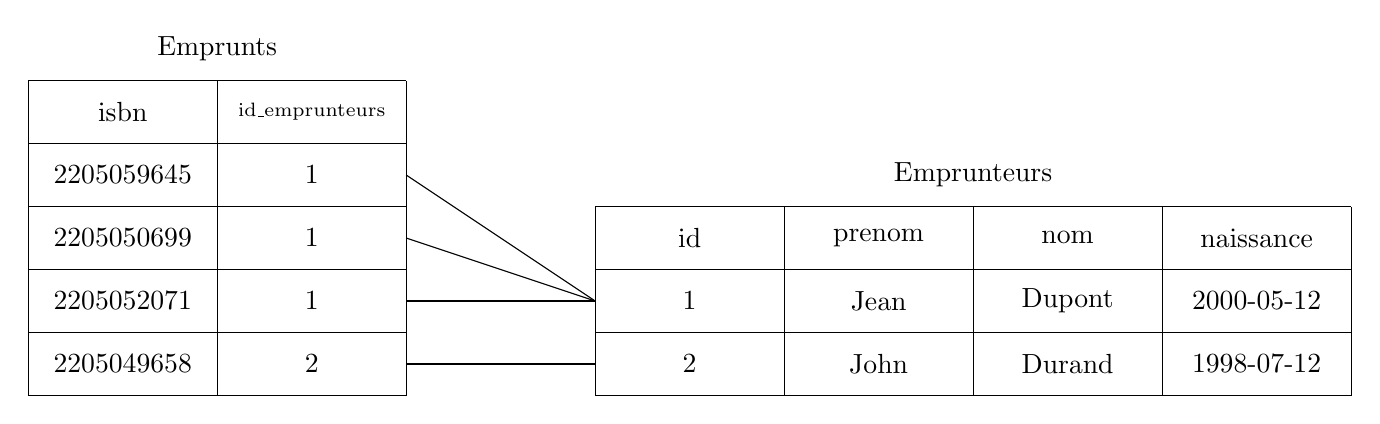
\begin{tikzpicture}[scale=0.8]
\node at (3,5.5) {Emprunts};
\draw (0,0) grid[xstep=3] (6,5);
\node at (1.5,4.5) {isbn};
\node at (4.5,4.5) {\scriptsize id\_emprunteurs};

\node at (1.5,3.5) {2205059645};
\node at (1.5,1.5) {2205052071};
\node at (1.5,2.5) {2205050699};
\node at (1.5,0.5) {2205049658};
\node at (4.5,0.5) {2};
\node at (4.5,2.5) {1};
\node at (4.5,1.5) {1};
\node at (4.5,3.5) {1};

\node at (15,3.5) {Emprunteurs};

\draw (9,0) grid[xstep=3] (21,3);
\node at (10.5,2.5) {id};
\node at (13.5,2.5) {prenom};
\node at (16.5,2.5) {nom};
\node at (19.5,2.5) {naissance};

\node at (10.5,1.5) {1};
\node at (10.5,0.5) {2};
\node at (13.5,1.5) {Jean};
\node at (13.5,0.5) {John};
\node at (16.5,1.5) {Dupont};
\node at (16.5,0.5) {Durand};
\node at (19.5,1.5) {2000-05-12};
\node at (19.5,0.5) {1998-07-12};

\draw (6,3.5) --(9,1.5);
\draw (6,2.5) --(9,1.5);
\draw (6,1.5) --(9,1.5);
\draw (6,0.5) --(9,0.5);

\end{tikzpicture}
\captionof{figure}{Jointure des tables \emph{Emprunts} et \emph{Emprunteurs}}
\label{jointure}
\end{center}

La jointure crée un \emph{table temporaire} qui contient l'ensemble des données (figure \ref{virtuelle}).
\begin{center}
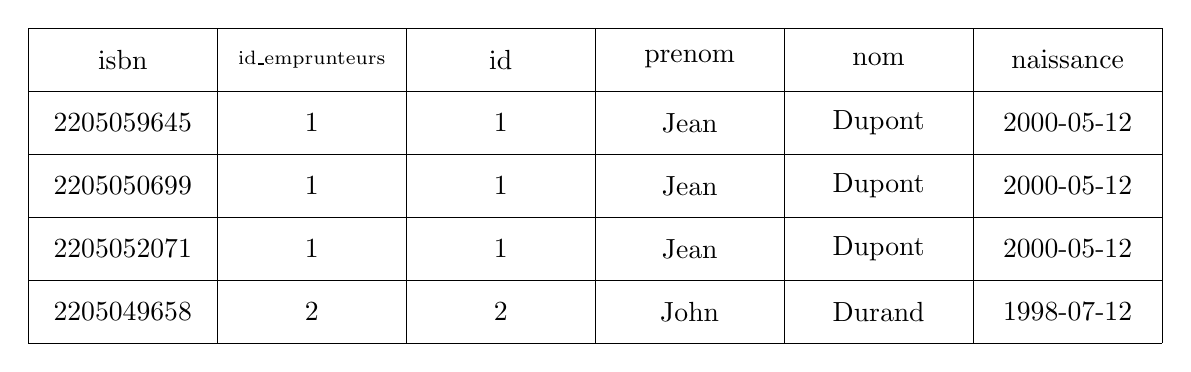
\begin{tikzpicture}[scale=0.8]
\draw (0,0) grid[xstep=3] (18,5);
\node at (1.5,4.5) {isbn};
\node at (4.5,4.5) {\scriptsize id\_emprunteurs};
\node at (7.5,4.5) {id};
\node at (10.5,4.5) {prenom};
\node at (13.5,4.5) {nom};
\node at (16.5,4.5) {naissance};

\node at (1.5,3.5) {2205059645};
\node at (1.5,1.5) {2205052071};
\node at (1.5,2.5) {2205050699};
\node at (1.5,0.5) {2205049658};

\node at (4.5,0.5) {2};
\node at (4.5,2.5) {1};
\node at (4.5,1.5) {1};
\node at (4.5,3.5) {1};

\node at (7.5,3.5) {1};
\node at (7.5,2.5) {1};
\node at (7.5,1.5) {1};
\node at (7.5,0.5) {2};

\node at (10.5,3.5) {Jean};
\node at (10.5,2.5) {Jean};
\node at (10.5,1.5) {Jean};
\node at (10.5,0.5) {John};

\node at (13.5,3.5) {Dupont};
\node at (13.5,2.5) {Dupont};
\node at (13.5,1.5) {Dupont};
\node at (13.5,0.5) {Durand};

\node at (16.5,3.5) {2000-05-12};
\node at (16.5,2.5) {2000-05-12};
\node at (16.5,1.5) {2000-05-12};
\node at (16.5,0.5) {1998-07-12};

\end{tikzpicture}
\captionof{figure}{Jointure des tables \emph{Emprunts} et \emph{Emprunteurs}}
\label{virtuelle}
\end{center}
Il est alors possible de récupérer n'importe quelle information.\\
La requête \ref{jointurereq} renvoie le nom des emprunteurs associés aux ISBN des bandes dessinées empruntées.
\begin{center}
\begin{lstlisting}[language=SQL]
SELECT Emprunteurs.nom, Emprunts.isbn FROM Emprunts 
JOIN Emprunteurs ON Emprunts.id_emprunteurs = Emprunteurs.id;
\end{lstlisting}
\captionof{code}{Jointure}
\label{jointurereq}
\end{center}
\begin{aretenir}[Remarque]
Certaines tables peuvent avoir des attributs qui possèdent le même nom. Pour éviter les ambiguïtés, il est judicieux de nommer les attributs ainsi: \emph{table.attribut}.
\end{aretenir}
\begin{activite}
\begin{enumerate}
\item Tester la requête \ref{jointurereq}.
\item Modifier la requête \ref{jointurereq} pour ne renvoyer que les ISBN empruntés par Dupont.
\item Il est possible d'effectuer une jointure avec plus de deux tables. Modifier la requête précédente pour renvoyer le \emph{titre} des bandes dessinées empruntées par Dupont.
\item Le mot clé \emph{ORDER BY} permet de classer les résultats selon le critère donné (requête \ref{order}). Classer les résultats de la requête précédente par ordre de titre.
\begin{center}
\begin{lstlisting}[language=SQL]
SELECT editeur FROM Editeurs 
WHERE editeur LIKE "G%"
ORDER BY editeur;
\end{lstlisting}
\captionof{code}{Classement des éditeurs commençant par G}
\label{order}
\end{center}
\end{enumerate}
\end{activite}
\end{Form}
\end{document}